% Saryu, paper A, draft v1: the architecture, before any comparison against other models.
% Build:  cd paper && pdflatex main && bibtex main && pdflatex main && pdflatex main
\documentclass[10pt]{article}
\usepackage[margin=1in]{geometry}
\usepackage[T1]{fontenc}
\usepackage{lmodern}
\usepackage{amsmath,amssymb}
\usepackage{booktabs,xcolor,microtype,caption,subcaption,enumitem,graphicx,float}
\usepackage{tikz,pgfplots}
\pgfplotsset{compat=1.17}
\usepgfplotslibrary{fillbetween}
\usetikzlibrary{arrows.meta,positioning,calc,fit,backgrounds,decorations.pathreplacing,shapes.geometric}
\usepackage[colorlinks=true,linkcolor=blue!50!black,citecolor=blue!50!black,urlcolor=blue!50!black]{hyperref}

\newtheorem{proposition}{Proposition}
\newenvironment{proof}{\par\noindent\textit{Proof.}\ }{\hfill$\square$\par\medskip}
\newcommand{\R}{\mathbb{R}}
\newcommand{\bu}{\mathbf{u}}
\newcommand{\bh}{\mathbf{h}}
\newcommand{\bc}{\mathbf{c}}
\newcommand{\bz}{\mathbf{z}}
\newcommand{\be}{\mathbf{e}}
\newcommand{\by}{\mathbf{y}}

\definecolor{mixc}{HTML}{F4B183}
\definecolor{ffnc}{HTML}{9DC3E6}
\definecolor{normc}{HTML}{E2E2E2}
\definecolor{projc}{HTML}{C5E0B4}
\definecolor{statec}{HTML}{FFE699}
\definecolor{memc}{HTML}{D9C3E9}
\definecolor{accA}{HTML}{2E75B6}
\definecolor{accB}{HTML}{C00000}

\tikzset{
  blk/.style={draw, rounded corners=2pt, minimum height=6mm, inner sep=3pt, align=center, font=\small},
  arr/.style={-{Stealth[length=2mm]}, thick},
  op/.style={draw, circle, inner sep=0pt, minimum size=4.5mm, font=\small},
}

\title{\textbf{Saryu: a recurrent language model whose state is carried by Householder reflections}\\[4pt]
\large Technical report --- draft v1 (architecture; comparisons pending)}
\author{Varun Sharma}
\date{15 September 2026}

\begin{document}
\maketitle

\begin{abstract}
Saryu is a recurrent language model with a fixed-size state. Every layer keeps one small vector per
head, and every token moves that vector with two input-dependent Householder transforms
$I-\beta\bu\bu^\top$ before a gate writes new content into it. The transform strength is parameterised
as $\beta = 1-\cos\theta$, so it lives in $[0,2]$ by construction: $\beta=2$ is an exact, norm-preserving
reflection and a stationary point of the parameterisation, $\beta=1$ a projection, $\beta<1$ a
contraction. Because reflections do not commute, the state depends on the \emph{order} of the tokens,
which no diagonal (commuting) transport can express; because every transform has spectral norm at most one and
the write is convex, the state is provably bounded. The recurrence is trained with an exact
chunk-parallel kernel (an inverse-free triangular solve per chunk) and generates at a per-token cost
independent of context length. This draft describes the architecture, the kernel, the design
reasoning and the two models trained so far (5M and 25M parameters, character-level enwik8, trained
at context 128, and measured to use about 512 characters of context and no more). It reports only Saryu's own measurements;
matched comparisons against other architectures are the subject of the next version.
\end{abstract}

% ======================================================================================
\section{What Saryu is for}

A transformer re-reads its whole context for every token it writes; its memory grows with the
context. A recurrent model instead compresses the past into a state of fixed size and updates it once
per token, so the cost of writing token $t$ does not depend on $t$. The question for any recurrent
design is what that fixed state can \emph{represent}, and whether it can be trained in parallel.

Much recent work uses \emph{diagonal} (element-wise) recurrences, where each coordinate of the state
decays and is written independently~\cite{gu2023mamba}. Diagonal matrices commute, so the product of
the transitions is the same whatever order the tokens came in. That is a real restriction: such
models cannot track state through non-commuting operations without help~\cite{merrill2024,sarrof2024},
and allowing negative eigenvalues in the transition is one way to recover
it~\cite{grazzi2024}.

Saryu's position is that order should be carried by the state itself, cheaply. Its transition is a
product of Householder transforms~\cite{householder1958}: rank-one corrections of the identity, each
determined by one unit vector and one scalar. Two of them per token cost $O(d_h)$ per head, they can be
exact reflections (norm-preserving, eigenvalue $-1$), and two reflections about different mirrors do not
commute (Figure~\ref{fig:order}). The rest of the block is chosen so that this transport trains
stably and in parallel.

\paragraph{Contributions of this draft.}
\begin{enumerate}[leftmargin=*,itemsep=1pt]
  \item A recurrent block whose per-head \emph{vector} state is moved by input-dependent Householder
        transforms with $\beta=1-\cos\theta$, and written through a convex cosine gate
        (Section~\ref{sec:arch}).
  \item A boundedness guarantee for the state under any input (Proposition~\ref{prop:bounded}) and the
        commutativity argument for why the transport must not be diagonal
        (Section~\ref{sec:why}).
  \item An exact chunk-parallel training kernel with a log-space rescaling that keeps it finite
        (Section~\ref{sec:kernel}).
  \item Two trained character-level models and a description of what their transports learned
        (Section~\ref{sec:results}).
\end{enumerate}

% ======================================================================================
\section{Architecture}
\label{sec:arch}

\subsection{The transport: one Householder transform}

For a unit vector $\bu\in\R^{d_h}$ and a scalar $\beta$, the generalised Householder transform is
\begin{equation}
  H(\bu,\beta) = I - \beta\,\bu\bu^\top .
\end{equation}
It leaves every vector orthogonal to $\bu$ unchanged and multiplies the component along $\bu$ by
$1-\beta$. So $\beta$ selects a regime (Figure~\ref{fig:reflection}, left):
$\beta=0$ is the identity, $\beta\in(0,1)$ shrinks the component along $\bu$, $\beta=1$ deletes it
(a projection), and $\beta=2$ flips its sign --- a reflection through the hyperplane $\bu^\perp$, which is
orthogonal and preserves the norm exactly.

Saryu parameterises the strength through an angle,
\begin{equation}
  \beta = 1-\cos\theta, \qquad 1-\beta = \cos\theta \in[-1,1],
  \label{eq:beta}
\end{equation}
so the eigenvalue along $\bu$ is literally $\cos\theta$. Three properties follow
(Figure~\ref{fig:reflection}, right). The range $[0,2]$ holds for every $\theta$, so no input can push
the transform outside it. The reflection $\beta=2$ is reached \emph{exactly}, at $\theta=\pi$ (a
sigmoid $2\sigma(x)$ only approaches it). And $d\beta/d\theta=\sin\theta$ vanishes there, so a reflection
is a stationary point that training does not drift away from by accident, while $\beta$ can still move
when the data asks for a contraction. The bias of the angle projection is initialised to $\pi$ with
zero weights, so every transform starts as an exact reflection.

\begin{figure}[t]
\centering
\begin{minipage}[c]{0.46\linewidth}\centering
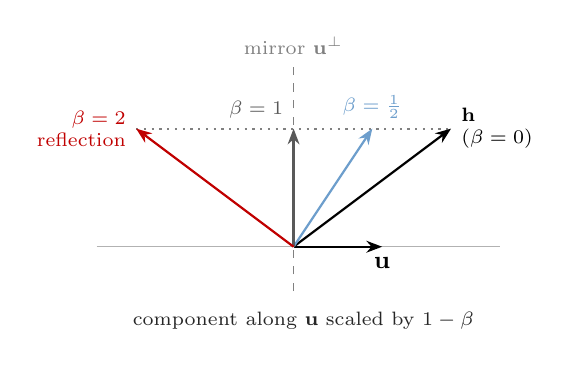
\begin{tikzpicture}[scale=1.25]
  \draw[dashed, gray] (0,-0.45) -- (0,1.85) node[above, font=\scriptsize] {mirror $\bu^\perp$};
  \draw[gray!60] (-2.0,0) -- (2.1,0);
  \draw[arr, black] (0,0) -- (0.9,0) node[below, font=\small] {$\bu$};
  \draw[dotted, thick, gray] (-1.6,1.2) -- (1.6,1.2);
  \draw[arr, black] (0,0) -- (1.6,1.2) node[right, font=\scriptsize, align=left] {$\bh$\\($\beta=0$)};
  \draw[arr, accA!70] (0,0) -- (0.8,1.2) node[above, font=\scriptsize] {$\beta=\tfrac12$};
  \draw[arr, gray!70!black] (0,0) -- (0,1.2) node[above left, font=\scriptsize] {$\beta=1$};
  \draw[arr, accB] (0,0) -- (-1.6,1.2) node[left, font=\scriptsize, align=right] {$\beta=2$\\reflection};
  \node[font=\scriptsize, gray!30!black] at (0.1,-0.75) {component along $\bu$ scaled by $1-\beta$};
\end{tikzpicture}
\end{minipage}\hfill
\begin{minipage}[c]{0.5\linewidth}\centering
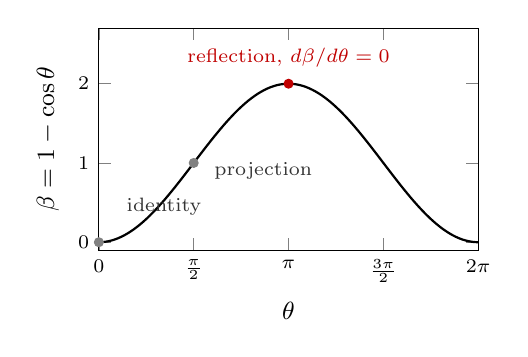
\begin{tikzpicture}
\begin{axis}[width=6.4cm, height=4.4cm, xmin=0, xmax=6.2832, ymin=-0.1, ymax=2.7,
  xtick={0,1.5708,3.1416,4.7124,6.2832}, xticklabels={$0$,$\frac{\pi}{2}$,$\pi$,$\frac{3\pi}{2}$,$2\pi$},
  ytick={0,1,2}, xlabel={$\theta$}, ylabel={$\beta=1-\cos\theta$},
  tick label style={font=\scriptsize}, label style={font=\small}]
  \addplot[domain=0:6.2832, samples=120, thick, black] {1-cos(deg(x))};
  \addplot[only marks, mark=*, mark size=1.6pt, accB] coordinates {(3.1416,2)};
  \addplot[only marks, mark=*, mark size=1.6pt, gray] coordinates {(1.5708,1) (0,0)};
  \node[font=\scriptsize, accB, anchor=south] at (axis cs:3.1416,2.08) {reflection, $d\beta/d\theta=0$};
  \node[font=\scriptsize, gray!40!black, anchor=west] at (axis cs:1.75,0.9) {projection};
  \node[font=\scriptsize, gray!40!black, anchor=west] at (axis cs:0.3,0.45) {identity};
\end{axis}
\end{tikzpicture}
\end{minipage}
\caption{\textbf{Left:} one Householder transform $I-\beta\bu\bu^\top$ applied to a state $\bh$. Only the
component along $\bu$ changes; at $\beta=2$ the state is mirrored and its norm is unchanged.
\textbf{Right:} the parameterisation $\beta=1-\cos\theta$ is bounded in $[0,2]$ and has zero slope at the
exact reflection $\theta=\pi$.}
\label{fig:reflection}
\end{figure}

\subsection{One recurrent step}

Each layer has $H=8$ heads with state $\bh\in\R^{d_h}$, $d_h=d/H$. For token $t$ the layer computes, per
head, $n_h=2$ unit vectors $\bu_{t,1},\bu_{t,2}$, their strengths $\beta_{t,1},\beta_{t,2}$, a scalar gate
$g_t$ and a content vector $\bc_t$, and updates
\begin{equation}
  \bh_t \;=\; a_t\, T_t\, \bh_{t-1} + \mathbf{b}_t, \qquad
  T_t = H(\bu_{t,2},\beta_{t,2})\,H(\bu_{t,1},\beta_{t,1}), \qquad
  a_t = 1-g_t,\quad \mathbf{b}_t = g_t\,\bc_t,
  \label{eq:step}
\end{equation}
with the gate again an angle,
\begin{equation}
  g_t = \min\!\Big(\tfrac{1-\cos\varphi_t}{2},\; 0.9\Big)\in[0,0.9].
\end{equation}
The gate is a single scalar per head: $a_t$ close to one keeps the transported past, $g_t$ close to one
replaces it with new content. The cap at $0.9$ keeps $a_t\ge 0.1$, which the training kernel relies on
(Section~\ref{sec:kernel}). Figure~\ref{fig:step} draws the step.

\begin{figure}[t]
\centering
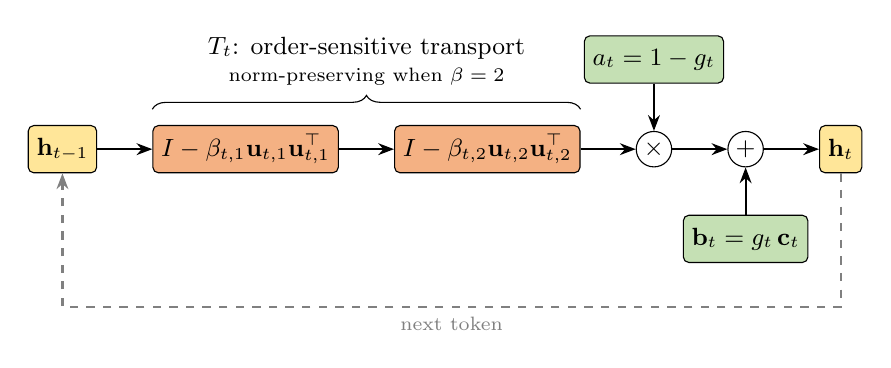
\begin{tikzpicture}[node distance=7mm]
  \node[blk, fill=statec] (h0) {$\bh_{t-1}$};
  \node[blk, fill=mixc, right=of h0] (H1) {$I-\beta_{t,1}\bu_{t,1}\bu_{t,1}^\top$};
  \node[blk, fill=mixc, right=of H1] (H2) {$I-\beta_{t,2}\bu_{t,2}\bu_{t,2}^\top$};
  \node[op, right=of H2] (mul) {$\times$};
  \node[op, right=of mul] (add) {$+$};
  \node[blk, fill=statec, right=of add] (h1) {$\bh_t$};
  \draw[arr] (h0) -- (H1); \draw[arr] (H1) -- (H2); \draw[arr] (H2) -- (mul);
  \draw[arr] (mul) -- (add); \draw[arr] (add) -- (h1);
  \node[blk, fill=projc, above=6mm of mul] (a) {$a_t=1-g_t$};
  \node[blk, fill=projc, below=6mm of add] (b) {$\mathbf{b}_t=g_t\,\bc_t$};
  \draw[arr] (a) -- (mul); \draw[arr] (b) -- (add);
  \draw[decorate, decoration={brace, amplitude=5pt}] ($(H1.north west)+(0,2mm)$) -- ($(H2.north east)+(0,2mm)$)
    node[midway, above=5pt, font=\small, align=center] {$T_t$: order-sensitive transport\\[-1pt]
    {\scriptsize norm-preserving when $\beta=2$}};
  \draw[arr, dashed, gray] (h1.south) -- ++(0,-17mm) -| node[pos=0.25, below, font=\scriptsize] {next token} (h0.south);
\end{tikzpicture}
\caption{One recurrent step of one head (Eq.~\ref{eq:step}). All of $\bu,\beta,g,\bc$ are computed from
the current token's features, so the transport is input-dependent. The state is a vector of
$d_h=d/8$ numbers.}
\label{fig:step}
\end{figure}

\subsection{The block and the model}

The recurrence sits inside a gated block (Figure~\ref{fig:arch}, right). The input is normalised with
LayerNorm~\cite{ba2016} and passed through a depthwise causal convolution of width 4, giving features
$\bz_t$ that see the last four tokens. Linear projections of $\bz_t$ give the reflection vectors
(normalised to unit length per head), the angles $\theta$ and $\varphi$, and the content $\bc_t$. The
per-head outputs of the recurrence are normalised with RMSNorm~\cite{zhang2019rms}, multiplied by a
SiLU~\cite{elfwing2018} output gate computed from $\bz_t$, and projected back to width $d$.

The language model (Figure~\ref{fig:arch}, left) stacks $N$ layers, each a Saryu block followed by a
SwiGLU feed-forward block~\cite{shazeer2020} of hidden width $2d$, both residual and pre-normalised. An
optional \emph{value embedding} --- a second token embedding added to the content $\bc_t$ of every
block --- is used in the 5M model. A final LayerNorm and a linear head give next-character logits.

A Saryu block has about $5d^2$ parameters (reflection vectors $2d^2$; content, output gate and output
projections $d^2$ each) and a SwiGLU block $6d^2$.

\begin{figure}[t]
\centering
\begin{minipage}[b]{0.3\linewidth}\centering
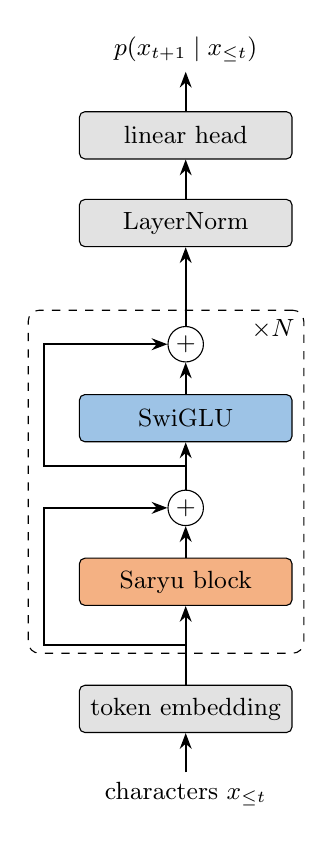
\begin{tikzpicture}[node distance=5mm]
  \node[font=\small] (tok) {characters $x_{\le t}$};
  \node[blk, fill=normc, above=of tok, minimum width=27mm] (emb) {token embedding};
  \node[blk, fill=mixc, above=10mm of emb, minimum width=27mm] (mix) {Saryu block};
  \node[op, above=4mm of mix] (r1) {$+$};
  \node[blk, fill=ffnc, above=6mm of r1, minimum width=27mm] (ffn) {SwiGLU};
  \node[op, above=4mm of ffn] (r2) {$+$};
  \node[blk, fill=normc, above=10mm of r2, minimum width=27mm] (lnf) {LayerNorm};
  \node[blk, fill=normc, above=of lnf, minimum width=27mm] (head) {linear head};
  \node[font=\small, above=of head] (out) {$p(x_{t+1}\mid x_{\le t})$};
  \draw[arr] (tok) -- (emb);
  \coordinate (s1) at ($(emb.north)+(0,5mm)$);
  \coordinate (s2) at ($(r1.north)+(0,3mm)$);
  \draw[arr] (emb) -- (mix); \draw[arr] (mix) -- (r1); \draw[arr] (r1) -- (ffn);
  \draw[arr] (ffn) -- (r2); \draw[arr] (r2) -- (lnf); \draw[arr] (lnf) -- (head); \draw[arr] (head) -- (out);
  \draw[arr] (s1) -- ++(-18mm,0) |- (r1.west);
  \draw[arr] (s2) -- ++(-18mm,0) |- (r2.west);
  \begin{scope}[on background layer]
    \node[draw, dashed, rounded corners, fit={($(s1)+(-20mm,-1mm)$) ($(r2.north)+(15mm,2mm)$)},
      inner sep=0pt, label={[font=\small, anchor=north east]north east:$\times N$}] {};
  \end{scope}
\end{tikzpicture}
\end{minipage}\hfill
\begin{minipage}[b]{0.66\linewidth}\centering
\resizebox{\linewidth}{!}{%
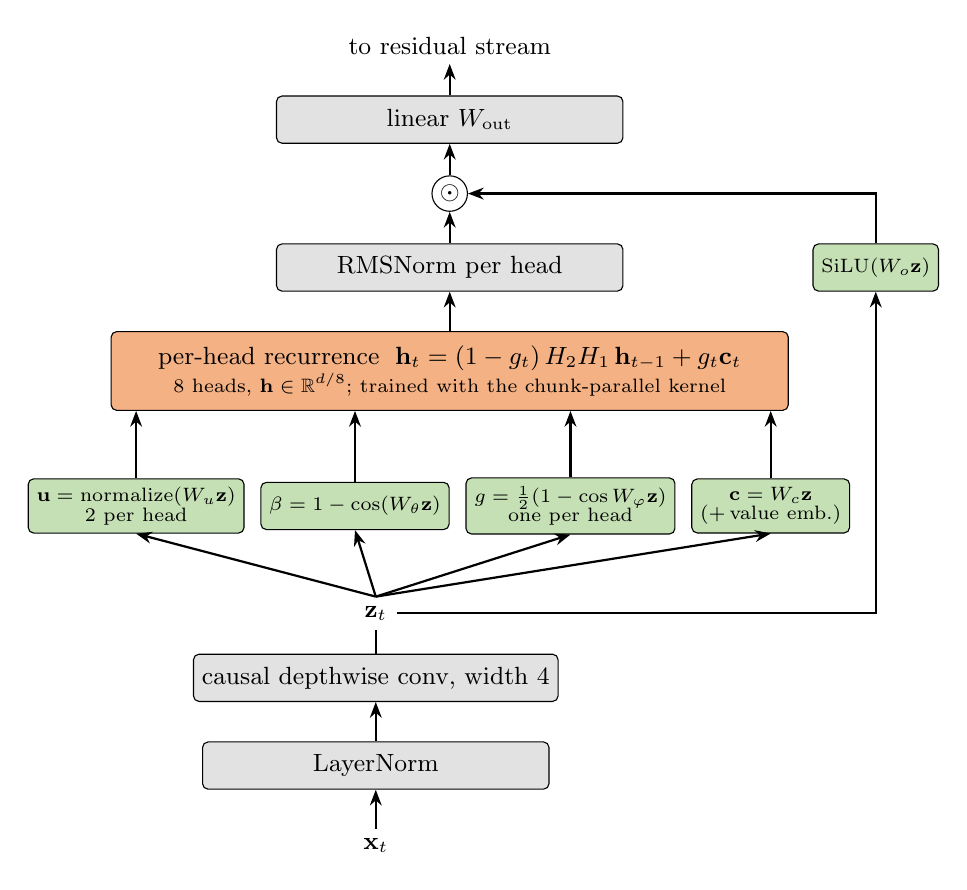
\begin{tikzpicture}[node distance=5mm]
  \node[font=\small] (x) {$\mathbf{x}_t$};
  \node[blk, fill=normc, above=of x, minimum width=44mm] (ln) {LayerNorm};
  \node[blk, fill=normc, above=of ln, minimum width=44mm] (conv) {causal depthwise conv, width 4};
  \node[font=\small, above=3mm of conv] (z) {$\bz_t$};
  \node[blk, fill=projc, above left=8mm and 14mm of z, font=\scriptsize] (pu) {$\bu=\mathrm{normalize}(W_u\bz)$\\[-1pt]$2$ per head};
  \node[blk, fill=projc, right=2mm of pu, font=\scriptsize] (pb) {$\beta=1-\cos(W_\theta\bz)$};
  \node[blk, fill=projc, right=2mm of pb, font=\scriptsize] (pg) {$g=\tfrac12(1-\cos W_\varphi\bz)$\\[-1pt]one per head};
  \node[blk, fill=projc, right=2mm of pg, font=\scriptsize] (pc) {$\bc=W_c\bz$\\[-1pt]$(+\,\text{value emb.})$};
  \node[blk, fill=mixc, above=9mm of pb.north east, anchor=south, minimum width=86mm, minimum height=10mm] (rec)
    {per-head recurrence $\;\bh_t=(1-g_t)\,H_2H_1\,\bh_{t-1}+g_t\bc_t$\\[-1pt]
     {\scriptsize 8 heads, $\bh\in\R^{d/8}$; trained with the chunk-parallel kernel}};
  \node[blk, fill=normc, above=of rec, minimum width=44mm] (rms) {RMSNorm per head};
  \node[op, above=4mm of rms] (gate) {$\odot$};
  \node[blk, fill=normc, above=4mm of gate, minimum width=44mm] (outp) {linear $W_{\mathrm{out}}$};
  \node[font=\small, above=4mm of outp] (y) {to residual stream};
  \node[blk, fill=projc, font=\scriptsize, right=24mm of rms] (og) {$\mathrm{SiLU}(W_o\bz)$};
  \draw[arr] (x) -- (ln); \draw[arr] (ln) -- (conv); \draw[thick] (conv) -- (z);
  \foreach \p in {pu,pb,pg,pc} { \draw[arr] (z.north) -- (\p.south); \draw[arr] (\p.north) -- (\p.north |- rec.south); }
  \draw[arr] (rec) -- (rms); \draw[arr] (rms) -- (gate); \draw[arr] (gate) -- (outp); \draw[arr] (outp) -- (y);
  \draw[arr] (z.east) -| (og.south);
  \draw[arr] (og.north) |- (gate.east);
\end{tikzpicture}}
\end{minipage}
\caption{\textbf{Left:} the language model. Each of the $N$ layers is a Saryu block and a SwiGLU block,
both residual. The optional value embedding (a second token embedding) enters every Saryu block through
its content $\bc_t$. \textbf{Right:} the Saryu block. The convolution gives every projection a short local
window; the recurrence carries everything older. At generation time each layer carries $d$ recurrent
numbers ($8$ heads $\times\,d/8$) plus the convolution's last three inputs.}
\label{fig:arch}
\end{figure}

\subsection{Generation cost}

At generation time a layer holds its $H$ head states ($d$ numbers in total) and the last three inputs of
the convolution ($3d$ numbers). For the 25M model ($d=744$, four layers) that is $11{,}904$ numbers for
the whole network, whether the context so far is ten characters or ten million, and each new token costs
one pass through the layers. There is no cache that grows with the context.

% ======================================================================================
\section{Why the transport is built this way}
\label{sec:why}

\subsection{Order: diagonal transports cannot see it}

If every transition matrix commutes with every other --- as diagonal or element-wise transitions
do~\cite{gu2023mamba} --- then a pure transport $\bh_T = T_{x_T}\cdots T_{x_1}\bh_0$ is the same for every
ordering of the same tokens: the state is a function of the \emph{multiset} of inputs. The best accuracy
any such model can reach on a task is therefore bounded by the best function of the multiset, a number
that can be computed exactly by enumeration. On the word problem of the symmetric group $S_3$ at length 8
that bound is $0.385$ (chance is $0.167$), while for the cyclic group $\mathbb{Z}_6$ of the same order it is
$1.0$, because there the multiset determines the answer.

In a small experiment with a width-64 transport, two commuting transports (a diagonal rotation and a
single fixed Givens pairing) reached $0.388\pm0.006$ and $0.389\pm0.003$ on $S_3$ --- on the bound --- and
$1.000$ on $\mathbb{Z}_6$; a non-commuting transport (alternating Givens pairings) reached
$0.779\pm0.380$ on $S_3$ over three seeds, above the bound that no commuting transport can
cross.\footnote{Repository \texttt{evidence/ceiling.py}, log \texttt{evidence/results/v2.txt}. The
non-commuting arm there is a Givens butterfly, not Saryu's reflections; the experiment establishes the
ceiling, not Saryu's accuracy.} Two reflections about different mirrors already fail to commute
(Figure~\ref{fig:order}): in the plane they compose to rotations by $+90^\circ$ and $-90^\circ$.

This is the same observation that motivates negative eigenvalues~\cite{grazzi2024} and products of
Householder transforms~\cite{siems2025} in matrix-state linear recurrences. By the Cartan--Dieudonn\'e
theorem every orthogonal $d_h\times d_h$ matrix is a product of at most $d_h$ reflections; with $n_h=2$ per
token a single step is a reflection pair (at $\beta=2$, a rotation in one plane), and longer products are
built up across tokens.

\begin{figure}[t]
\centering
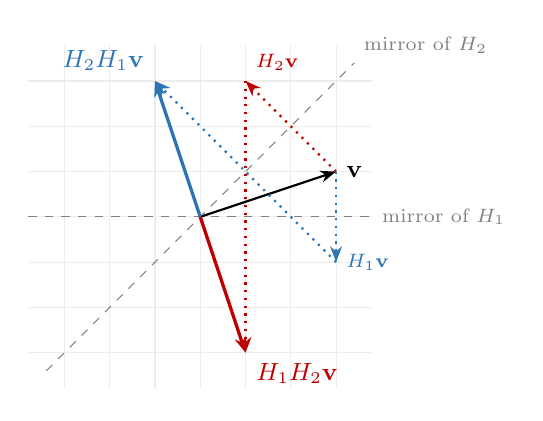
\begin{tikzpicture}[scale=1.15]
  \draw[step=0.5, gray!15] (-1.9,-1.9) grid (1.9,1.9);
  \draw[dashed, gray] (-1.9,0) -- (1.9,0) node[right, font=\scriptsize] {mirror of $H_1$};
  \draw[dashed, gray] (-1.7,-1.7) -- (1.7,1.7) node[above right, font=\scriptsize] {mirror of $H_2$};
  \draw[arr, black] (0,0) -- (1.5,0.5) node[right, font=\small] {$\mathbf{v}$};
  % H1 then H2
  \draw[arr, accA, dotted] (1.5,0.5) -- (1.5,-0.5) node[right, font=\scriptsize] {$H_1\mathbf{v}$};
  \draw[arr, accA, dotted] (1.5,-0.5) -- (-0.5,1.5);
  \draw[arr, accA, very thick] (0,0) -- (-0.5,1.5) node[above left, font=\small] {$H_2H_1\mathbf{v}$};
  % H2 then H1
  \draw[arr, accB, dotted] (1.5,0.5) -- (0.5,1.5) node[above right, font=\scriptsize] {$H_2\mathbf{v}$};
  \draw[arr, accB, dotted] (0.5,1.5) -- (0.5,-1.5);
  \draw[arr, accB, very thick] (0,0) -- (0.5,-1.5) node[below right, font=\small] {$H_1H_2\mathbf{v}$};
\end{tikzpicture}
\caption{Order sensitivity. The same two reflections applied to the same state in opposite orders give
different states ($H_2H_1$ is a rotation by $+90^\circ$, $H_1H_2$ by $-90^\circ$). A recurrence built from
them can tell ``$a$ then $b$'' from ``$b$ then $a$'' through the transport itself; a diagonal transport,
whose factors commute, cannot.}
\label{fig:order}
\end{figure}

\subsection{Stability: the state cannot blow up}

\begin{proposition}
\label{prop:bounded}
If $\beta\in[0,2]$ for every transform and $g_t\in[0,1]$, then for every input sequence
\[ \|\bh_t\| \;\le\; \max\big(\|\bh_0\|,\ \max_{s\le t}\|\bc_s\|\big). \]
\end{proposition}
\begin{proof}
$H(\bu,\beta)$ is symmetric with eigenvalues $1$ (on $\bu^\perp$) and $1-\beta\in[-1,1]$ (on $\bu$), so its
spectral norm is at most one, and so is that of $T_t$. Then
$\|\bh_t\|\le(1-g_t)\|\bh_{t-1}\|+g_t\|\bc_t\|\le\max(\|\bh_{t-1}\|,\|\bc_t\|)$, and the claim follows by
induction.
\end{proof}

The bound is what the cosine parameterisation buys. An unconstrained $\beta$ can leave $[0,2]$ and make
$|1-\beta|>1$, after which the state grows geometrically with length; in our early single-layer
experiments an unbounded $\beta$ produced state norms above $4\times10^5$ at length 4096. With
Eq.~\ref{eq:beta} the bound holds whatever the weights are.

\subsection{Why not a sigmoid, and why not a fixed reflection}

A fixed $\beta=2$ makes every step orthogonal but removes the model's ability to forget along a
direction, and it fixes $\det T_t=(-1)^{n_h}$ for every token. A sigmoid $\beta=2\sigma(x)$ can approach a
reflection but never reach it. In small state-tracking experiments on the groups $S_4$ and $A_4$ with
$n_h\in\{2,3\}$ (four seeds per cell, sixteen runs per parameterisation), the sigmoid solved $0$ of $16$
runs and settled near $\beta\approx1$ (a projection); $1-\cos\theta$ solved $9$ of $16$, reaching
$\beta=2.000$ where an exact reflection was consistent with the group and moving away from it where it was
not.\footnote{Repository \texttt{evidence/beta\_activation.py}. These are toy experiments with a single
transport layer and are reported here only as the reason for the design choice.}

% ======================================================================================
\section{Training in parallel: the chunkwise kernel}
\label{sec:kernel}

Eq.~\ref{eq:step} is sequential. Training it token by token would cost one Python-level step per token.
Saryu instead processes chunks of $C=8$ tokens at once, exactly, using the structure of Householder
products~\cite{bischof1987}; the approach follows the chunkwise delta-rule kernels of
\cite{yang2024delta}, adapted to a vector state with an interleaved gated write.

\paragraph{Removing the gate.} Within a chunk, let $\alpha_t=\prod_{k\le t}a_k$ ($\alpha_0=1$) and rescale
$\mathbf{s}_t=\bh_t/\alpha_t$. Eq.~\ref{eq:step} becomes $\mathbf{s}_t=T_t\mathbf{s}_{t-1}+\be_t$ with
$\be_t=\mathbf{b}_t/\alpha_t$ and $\be_0=\bh_0$, the state carried in from the previous chunk. The gate
has disappeared into the injections.

\paragraph{Unrolling the reflections.} Number the $R=Cn_h$ transforms of the chunk $r=1,\dots,R$ in the
order they are applied, and let $\tau(r)$ be the token that transform $r$ belongs to. Each transform
subtracts $\beta_r y_r\bu_r$ from the running vector, where $y_r$ is $\bu_r^\top$ of that vector just
before transform $r$. The running vector at that moment is the sum of injections so far minus the
earlier corrections, which gives
\begin{equation}
  y_r + \sum_{r'<r}\beta_{r'}\,(\bu_r^\top\bu_{r'})\,y_{r'} \;=\; \bu_r^\top\!\!\sum_{j<\tau(r)}\be_j ,
  \qquad\text{i.e.}\qquad
  \big(I+\operatorname{tril}(G\,\mathrm{diag}(\beta),-1)\big)\,\by = \mathbf{r},
  \label{eq:tri}
\end{equation}
with Gram matrix $G_{rr'}=\bu_r^\top\bu_{r'}$. The system is unit lower triangular, so $\by$ comes from
one triangular solve with no matrix inverse. All $C$ outputs of the chunk then follow at once:
\begin{equation}
  \bh_t \;=\; \alpha_t\Big(\sum_{j\le t}\be_j \;-\; \sum_{r:\,\tau(r)\le t}\beta_r\,y_r\,\bu_r\Big),
  \qquad t=1,\dots,C.
  \label{eq:chunkout}
\end{equation}

\begin{figure}[t]
\centering
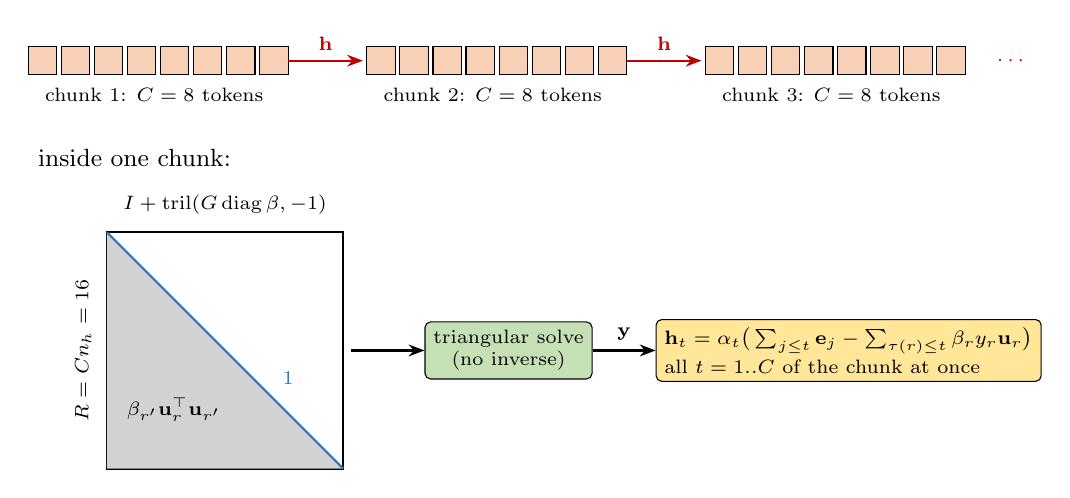
\begin{tikzpicture}
  % chunks
  \foreach \c/\x in {0/0,1/4.3,2/8.6} {
    \foreach \i in {0,...,7} { \draw[fill=mixc!60] (\x+\i*0.42,0) rectangle ++(0.36,0.36); }
    \node[font=\scriptsize] at (\x+1.6,-0.25) {chunk \pgfmathparse{int(\c+1)}\pgfmathresult: $C=8$ tokens};
  }
  \draw[arr, accB] (3.3,0.18) -- (4.25,0.18) node[midway, above, font=\scriptsize] {$\bh$};
  \draw[arr, accB] (7.6,0.18) -- (8.55,0.18) node[midway, above, font=\scriptsize] {$\bh$};
  \node[font=\scriptsize, accB] at (12.5,0.18) {$\cdots$};
  \node[font=\small, anchor=west] at (0,-1.05) {inside one chunk:};
  % zoom
  \begin{scope}[shift={(1.0,-5.0)}]
    \draw[thick] (0,0) rectangle (3,3);
    \fill[gray!35] (0,3) -- (0,0) -- (3,0) -- cycle;
    \draw[thick, accA] (0,3) -- (3,0);
    \node[font=\scriptsize, align=center] at (1.5,3.35) {$I+\operatorname{tril}(G\,\mathrm{diag}\,\beta,-1)$};
    \node[font=\scriptsize] at (0.85,0.75) {$\beta_{r'}\bu_r^\top\bu_{r'}$};
    \node[font=\scriptsize, accA] at (2.3,1.15) {$1$};
    \node[font=\scriptsize, rotate=90] at (-0.3,1.5) {$R=Cn_h=16$};
  \end{scope}
  \node[blk, fill=projc, font=\scriptsize] (solve) at (6.1,-3.5) {triangular solve\\(no inverse)};
  \draw[arr] (4.1,-3.5) -- (solve.west);
  \node[blk, fill=statec, font=\scriptsize, right=8mm of solve, align=left] (outs)
    {$\bh_t=\alpha_t\big(\sum_{j\le t}\be_j-\sum_{\tau(r)\le t}\beta_r y_r\bu_r\big)$\\[1pt]
     all $t=1..C$ of the chunk at once};
  \draw[arr] (solve) -- node[above, font=\scriptsize] {$\by$} (outs);
\end{tikzpicture}
\caption{The chunkwise kernel. The sequence is cut into chunks of $C=8$ tokens and the state is carried
between chunks. Inside a chunk the $16$ transforms couple only through a unit lower-triangular system
(Eq.~\ref{eq:tri}); one solve yields every output of the chunk (Eq.~\ref{eq:chunkout}).}
\label{fig:kernel}
\end{figure}

\paragraph{Keeping it finite.} Computed naively, $\alpha_t$ is a product of gates and $1/\alpha_t$ in
$\be_t$ overflows when a chunk contains several strong writes. Every physical quantity is a ratio
$\alpha_t/\alpha_j\le1$, so the kernel works with $\log\alpha_t$ centred on its mean over the chunk. Each
step lowers $\log\alpha_t$ by at most $\ln 10$ (the gate cap gives $a_t\ge0.1$), so over $C=8$ steps no
value lies further than $\tfrac{1}{8}\sum_{k=1}^{7}k\ln10\approx8.1$ from the mean, and no rescaling
factor exceeds $e^{8.1}\approx3\times10^3$.

\paragraph{Exactness and cost.} The kernel reproduces the token-by-token recurrence to floating-point
precision: on a randomly initialised block the largest absolute difference is $4.8\times10^{-7}$ in
single precision, and the repository tests check lengths 8, 64 and 128. Per chunk it forms a
$16\times16$ Gram matrix and solves one triangular system per head; the loop over chunks is still
sequential, so a length-$L$ forward pass takes $L/8$ chunk steps rather than $L$ token steps. The current
implementation is plain PyTorch without a fused GPU kernel.

% ======================================================================================
\section{The models trained so far}
\label{sec:results}

\subsection{Data, training and evaluation}

Both models are trained on enwik8~\cite{hutter2006}, the first $10^8$ bytes of an English Wikipedia
dump, decoded as UTF-8 and modelled at the character level. Characters that occur at least 100 times form
the vocabulary (480 characters plus one id for everything else, 481 in total). The first 95\% of the
characters are used for training and the last 5\% for evaluation. This split and vocabulary are our own;
the numbers below are not comparable with published enwik8 results, which use a byte-level 90/5/5 split.

\begin{table}[t]
\centering
\footnotesize
\begin{tabular}{@{}lcc@{}}
\toprule
 & \textbf{Saryu 5M} (checkpoint shipped with the code) & \textbf{Saryu 25M} \\
\midrule
parameters & 5,016,097 & 25,183,861 \\
width $d$ / layers / heads / $n_h$ & 320 / 4 / 8 / 2 & 744 / 4 / 8 / 2 \\
head state $d_h$ & 40 & 93 \\
value embedding & yes & no \\
training context / batch & 128 / 48 & 128 / 48 \\
steps (characters seen) & 5,000 (30.7M) & 10,000 (61.4M) \\
optimiser & AdamW, lr $10^{-3}$, wd 0.01 & AdamW, lr $10^{-3}$, wd 0.01 (matrices) \\
schedule & one-cycle~\cite{smith2017}, 5\% warm-up & warmup--stable--decay~\cite{wen2024wsd} (5\% / 20\%) \\
other & embeddings $10\times$ lr; gate proj.\ $0.1\times$ lr & z-loss $10^{-4}$; output proj.\ scaled $1/\sqrt{2N}$ \\
gradient clipping & 1.0 & 1.0 \\
hardware, time per step & one T4 GPU, $\approx$0.2\,s & one T4 GPU, 0.50\,s \\
\bottomrule
\end{tabular}
\caption{The two trained models. Both use the same block (Section~\ref{sec:arch}); they differ in width,
the value embedding and the training recipe.}
\label{tab:config}
\end{table}

\paragraph{Evaluation.} Each number below is measured with the model reading a window of
$L\in\{128,512,2048,8192\}$ characters and scoring only the \emph{last 128} characters of the window,
over 64 windows drawn at random from the evaluation text (8,192 scored characters per number). Every
window \emph{ends} at the same 64 positions, so each context length scores exactly the same characters
with more or less text in front of them. (An earlier version of this draft drew the window starts
separately for each $L$; its columns scored different characters and were not comparable to each
other.) The unit is bits per character (bpc); lower is better.

\subsection{Results}

\begin{table}[t]
\centering
\small
\begin{tabular}{@{}lcccc@{}}
\toprule
 & \multicolumn{4}{c}{bits per character, context length $L$} \\
\cmidrule(l){2-5}
model & 128 & 512 & 2048 & 8192 \\
\midrule
Saryu 5M (checkpoint shipped with the code) & 1.671 & 1.586 & 1.586 & 1.586 \\
Saryu 25M & \textbf{1.535} & \textbf{1.433} & \textbf{1.433} & \textbf{1.433} \\
\bottomrule
\end{tabular}
\caption{Character-level results on our enwik8 split, scoring identical text at every context length.
Both models were trained at context 128. The columns beyond 512 repeat because the models stop using
context there (Section~\ref{sec:context}).}
\label{tab:bpc}
\end{table}

\begin{figure}[t]
\centering
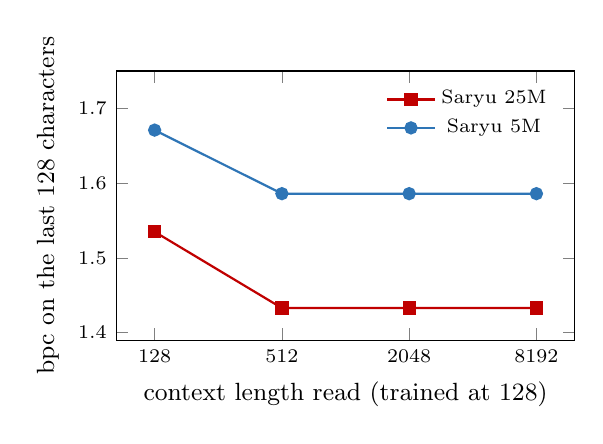
\begin{tikzpicture}
\begin{semilogxaxis}[width=7.4cm, height=5.0cm, log basis x=2,
  xtick={128,512,2048,8192}, xticklabels={128,512,2048,8192},
  xlabel={context length read (trained at 128)}, ylabel={bpc on the last 128 characters},
  ymin=1.39, ymax=1.75, legend style={font=\scriptsize, draw=none, fill=none}, legend pos=north east,
  tick label style={font=\scriptsize}, label style={font=\small}]
  \addplot[thick, mark=square*, accB] coordinates {(128,1.535) (512,1.433) (2048,1.433) (8192,1.433)};
  \addlegendentry{Saryu 25M}
  \addplot[thick, mark=*, accA] coordinates {(128,1.671) (512,1.586) (2048,1.586) (8192,1.586)};
  \addlegendentry{Saryu 5M}
\end{semilogxaxis}
\end{tikzpicture}\hfill
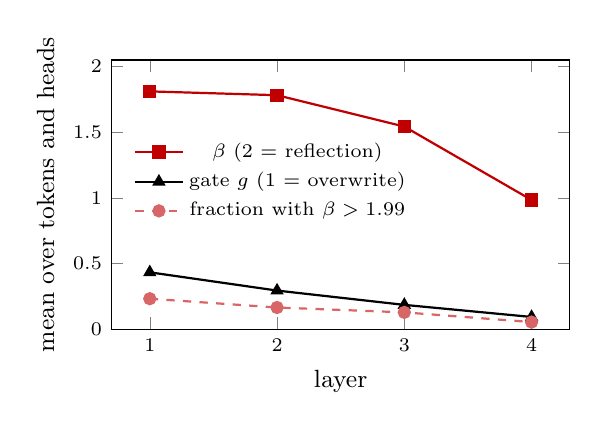
\begin{tikzpicture}
\begin{axis}[width=7.4cm, height=5.0cm, xtick={0,1,2,3}, xticklabels={1,2,3,4}, xlabel={layer},
  ymin=0, ymax=2.05, ylabel={mean over tokens and heads},
  legend style={font=\scriptsize, draw=none, fill=none, at={(0.03,0.55)}, anchor=west},
  tick label style={font=\scriptsize}, label style={font=\small}]
  \addplot[thick, mark=square*, accB] coordinates {(0,1.811) (1,1.782) (2,1.543) (3,0.984)};
  \addlegendentry{$\beta$ (2 = reflection)}
  \addplot[thick, mark=triangle*, black] coordinates {(0,0.433) (1,0.294) (2,0.185) (3,0.093)};
  \addlegendentry{gate $g$ (1 = overwrite)}
  \addplot[thick, dashed, mark=*, mark options={solid}, accB!60] coordinates {(0,0.232) (1,0.165) (2,0.128) (3,0.054)};
  \addlegendentry{fraction with $\beta>1.99$}
\end{axis}
\end{tikzpicture}
\caption{\textbf{Left:} bits per character against the context read, scoring identical text at every
length: both models flatten at 512 characters and never improve again. \textbf{Right:} what the 25M model's
transports do on evaluation text (four windows of 1,024 characters): lower layers are close to exact
reflections and rewrite often, the top layer uses softer transforms and rewrites rarely.}
\label{fig:results}
\end{figure}

Table~\ref{tab:bpc} and Figure~\ref{fig:results} (left) give the numbers. Three observations, stated
with the caution that this is a single corpus and small models:

\begin{itemize}[leftmargin=*,itemsep=2pt]
  \item \textbf{The models use about 512 characters of context and nothing before that.} Past 512 the
        state entering the scored text matches the long-context state to six decimals in every layer,
        the next-character distributions are unchanged ($\mathrm{KL}=0.000000$), and bpc stops moving
        (Section~\ref{sec:context}).
  \item \textbf{Context 128 is the only row that differs, for a mechanical reason.} At $L=128$ the
        scored characters have no context at all in front of them; the KL against the long-context
        predictions is $4.55$ at 5M and $8.39$ at 25M.
  \item \textbf{Scale helps.} Five times the parameters and twice the training characters lower bpc by
        about $0.15$ at every context length.
\end{itemize}

An earlier version of this draft reported $1.643\to1.467$ bpc from context 128 to 8192 at 25M and read
it as the model using context it was never trained on. Those numbers came from windows drawn separately
per length, so each column scored different text; the effect does not survive scoring identical text,
and the claim is withdrawn.

\subsection{How much context is used}
\label{sec:context}

Table~\ref{tab:bpc} flattens at 512, which could mean either that the extra text carries nothing or
that the model cannot see it. \texttt{evidence/effective\_context.py} separates the two by comparing,
at identical scored positions, the predictions and the recurrent state under context $L$ against the
longest context:

\begin{center}\small
\begin{tabular}{@{}rccc@{}}
\toprule
context & bpc & KL to 8192 & state cosine \\
\midrule
128 & 1.788326 & 4.553845 & --- \\
256 & 1.722210 & 0.015948 & 0.999525 \\
512 & 1.721628 & 0.000012 & 1.000000 \\
1024--8192 & 1.721638 & 0.000000 & 1.000000 \\
\bottomrule
\end{tabular}
\end{center}

(5M checkpoint, 16 windows; the 25M behaves the same, its 512-context state matching the 1024-context
state to $0.999996$.) Past 512 characters the state is not merely uninformative --- it is identical, so
the model cannot be using anything earlier. This follows from the architecture: the write is convex, so
the state is a decaying mixture, and with the measured mean gate of $0.09$ in the top layer,
$(1-0.09)^{512}\approx10^{-21}$. Reaching further needs a gate able to stay near zero for long spans, or
the separate fact memory of Section~\ref{sec:next}.

\subsection{What the transports learned}

Figure~\ref{fig:results} (right) summarises the 25M model's $\beta$ and gates on evaluation text; the
5M model shows the same pattern. In the first layer the mean $\beta$ is $1.81$ and $23\%$ of transforms
are exact reflections to within $0.01$, with only $4\%$ below $\beta=1$; the gate averages $0.43$, so the
state is rewritten substantially at most tokens; $15\%$ of first-layer gates sit at the $0.9$ cap, so the
cap does bind there. Moving up, both fall: in the fourth layer the mean
$\beta$ is $0.98$, half the transforms are contractions ($\beta<1$), and the mean gate is $0.09$, so the state
is kept for many tokens and edited softly. The model thus uses the full range the parameterisation allows
--- reflections with fast turnover low in the stack, gentle long-lived memory at the top --- rather than
collapsing to one regime.

% ======================================================================================
\section{Where Saryu goes next}
\label{sec:next}

\paragraph{Comparisons.} This draft deliberately reports no comparison. The next version will compare
Saryu with other architectures at matched parameters and training data --- a gated recurrent network
with the same block around it, matrix-state delta-rule models~\cite{yang2024delta,yang2024gated,siems2025}
and a transformer --- with several seeds, a second corpus,
state-tracking tasks, and throughput. The design questions above (Section~\ref{sec:why}) are
only settled once those numbers exist.

\paragraph{A fused kernel.} The chunkwise kernel is exact but written in plain PyTorch with a loop over
chunks. A fused GPU kernel is needed before training at larger scale.

\paragraph{A memory for facts.} Saryu's state is small by design: $d$ numbers per layer. That suits
tracking \emph{where} a sequence is, but it cannot store many independent facts, which is what
associative-recall tasks measure~\cite{arora2023zoology}. The intended full Saryu adds a matrix memory
next to the tracker (Figure~\ref{fig:memory}): a delta-rule store~\cite{yang2024delta} with $\beta<1$ (no
reflections inside the store, where a reflection would invert a superseded fact), addressed by content
bound to the tracked state. A first version exists but does not train: because the tracker moves at
every token, a fact written under one state is queried under a different one and the addresses never
match. The planned fix is a tracker that changes state only when a token should change it.

\begin{figure}[t]
\centering
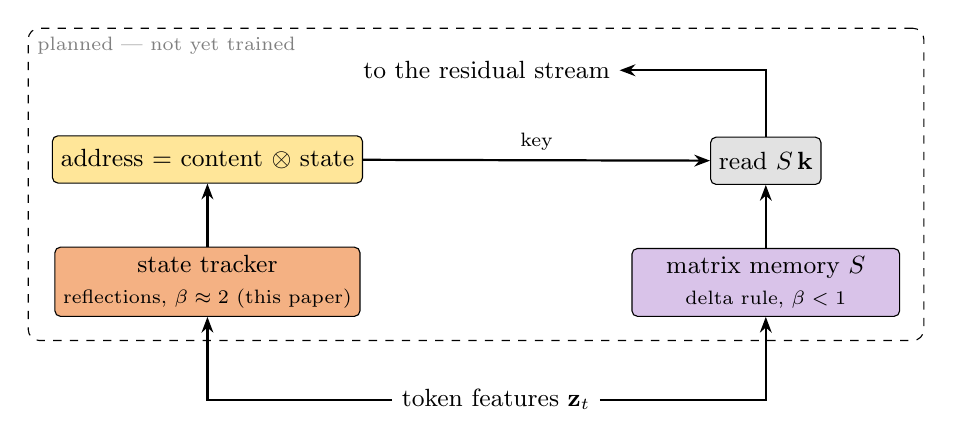
\begin{tikzpicture}[node distance=6mm]
  \node[font=\small] (x) {token features $\bz_t$};
  \node[blk, fill=mixc, above left=8mm and 4mm of x, minimum width=34mm] (trk) {state tracker\\{\scriptsize reflections, $\beta\approx2$ (this paper)}};
  \node[blk, fill=memc, above right=8mm and 4mm of x, minimum width=34mm] (mem) {matrix memory $S$\\{\scriptsize delta rule, $\beta<1$}};
  \node[blk, fill=statec, above=8mm of trk] (addr) {address = content $\otimes$ state};
  \node[blk, fill=normc, above=8mm of mem] (read) {read $S\,\mathbf{k}$};
  \coordinate (mid) at ($(addr.north)!0.5!(read.north)$);
  \node[font=\small, above=6mm of mid] (out) {to the residual stream};
  \draw[arr] (x) -| (trk); \draw[arr] (x) -| (mem);
  \draw[arr] (trk) -- (addr); \draw[arr] (addr) -- node[above, font=\scriptsize] {key} (read);
  \draw[arr] (mem) -- (read); \draw[arr] (read) |- (out);
  \begin{scope}[on background layer]
    \node[draw, dashed, rounded corners, fit=(trk)(mem)(addr)(read)(out), inner sep=3mm,
      label={[font=\scriptsize, gray, anchor=north west]north west:planned --- not yet trained}] {};
  \end{scope}
\end{tikzpicture}
\caption{The intended full Saryu layer: the reflection tracker of this paper plus a matrix memory for
facts, addressed by content bound to the tracked state. Not part of the trained models.}
\label{fig:memory}
\end{figure}

% ======================================================================================
\section{Related work}

\paragraph{Gated and linear recurrences.} LSTMs~\cite{hochreiter1997} and GRUs~\cite{cho2014} gate a
vector state through nonlinear updates that must be trained sequentially. Linear attention~\cite{katharopoulos2020}
and selective state-space models~\cite{gu2023mamba} make the recurrence linear in the state so it can be
trained in parallel, usually with diagonal transitions, which commute.

\paragraph{Orthogonal and Householder recurrences.} Unitary and orthogonal RNNs keep the transition
norm-preserving to avoid vanishing and exploding gradients~\cite{arjovsky2016}, and Householder
reflections are an efficient way to parameterise them~\cite{mhammedi2017}. In those models the transition
is a learned constant, the same for every token. Saryu's transforms are computed from the input at every
token, and $\beta$ lets each one be anything from the identity through a projection to a reflection.

\paragraph{Delta-rule models and state tracking.} DeltaNet~\cite{yang2024delta} and Gated
DeltaNet~\cite{yang2024gated} update a \emph{matrix} state with generalised Householder transforms of the
form $I-\beta\mathbf{k}\mathbf{k}^\top$ and write key--value outer products; extending $\beta$ to $[0,2]$
gives negative eigenvalues and state-tracking ability~\cite{grazzi2024}, and DeltaProduct applies several
such transforms per token~\cite{siems2025}. Saryu shares the Householder transport and the
several-per-token structure. It differs in carrying a small \emph{vector} per head rather than a matrix, in
separating the write into a convex scalar-gated addition instead of a key--value outer product, in the
$1-\cos\theta$ parameterisation that makes the exact reflection reachable and stationary, and in the
log-space chunk kernel that this write requires. The price is the small state discussed in
Section~\ref{sec:next}.

% ======================================================================================
\section{Limitations of this draft}

No comparison with any other model is reported. Both models are small and trained on one character-level
corpus with a non-standard split; nothing here says how Saryu behaves at the scale of modern language
models. Each bpc number comes from 8,192 scored characters, with different characters at each context
length. The toy experiments cited in Section~\ref{sec:why} use single transport layers and small groups.
The training kernel is exact but not yet fast.

\bibliographystyle{abbrv}
\bibliography{refs}

\end{document}
